\documentclass{article}
\usepackage[utf8]{inputenc}
\usepackage{cancel}
\usepackage{amsthm,amssymb,amsmath}
\usepackage{mathtools}
\usepackage{tikz}
\usetikzlibrary{calc}
\usetikzlibrary{positioning}
\usepackage{parskip}
\usepackage{float}
\newtheorem{theorem}{Theorem}[section]
\newtheorem{corollary}{Corollary}[theorem]
\newtheorem{lemma}[theorem]{Lemma}
\setlength{\parskip}{1em}
\newcommand{\NN}{\mathbb{N}}
\newcommand{\ZZ}{\mathbb{Z}}
\newcommand{\RR}{\mathbb{R}}
\newcommand{\QQ}{\mathbb{Q}}
\newcommand{\CC}{\mathbb{C}}

\title{MAT 4800 Homework \# 1}
\author{Noah Reef }
\date{Spring 2023}

\usepackage{natbib}
\usepackage{graphicx}

\begin{document}
\maketitle
\section*{Problem \#1}

\begin{figure}[H]
    \centering
    \begin{tikzpicture}
    \draw (0,0) -- node[below, pos=.5]{$a$}(4,0) -- node[right, pos=.5]{$a$}(4,4) -- (0,4) -- (0,0) ;

    \draw (0,0) -- node[below, pos=.5]{$x$}(1,0) -- node[right, pos=.5]{$x$}(1,1) -- (0,1) -- (0,0) ;

    \draw (0,3) -- (1,3) -- (1,4) -- (0,4) -- (0,3) ;

     \draw (3,3) -- (4,3) -- (4,4) -- (3,4) -- (3,3) ;

      \draw (3,0) -- (4,0) -- (4,1) -- (3,1) -- (3,0) ;
    
    \end{tikzpicture}

    
    \caption{$a \times a$ Square Paper}
    \label{fig:paper}
\end{figure}

\subsection*{Part a}
\begin{figure}[H]
    \centering
    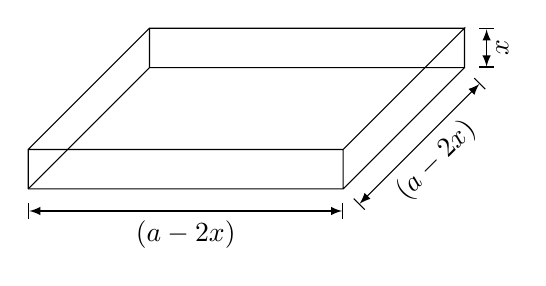
\begin{tikzpicture}[>=latex,scale=2]
    \pgfmathsetmacro{\x}{2}
    \pgfmathsetmacro{\y}{2}
    \pgfmathsetmacro{\z}{0.25}
    \path (0,0,\y) coordinate (A) (\x,0,\y) coordinate (B) (\x,0,0) coordinate (C) (0,0,0)
    coordinate (D) (0,\z,\y) coordinate (E) (\x,\z,\y) coordinate (F) (\x,\z,0) coordinate (G)
    (0,\z,0) coordinate (H);
    \draw (A)--(B)--(C)--(G)--(F)--(B) (A)--(E)--(F)--(G)--(H)--(E);
    \draw (A)--(D)--(C) (D)--(H);
    
    \draw[thin,|<->|] ($(A)+(0,-4pt)$) -- node[below]{$(a-2x)$}($(B)+(0,-4pt)$);
    \draw[thin,|<->|] ($(B)+(-45:4pt)$) -- node[below,sloped]{$(a-2x)$}($(C)+(-45:4pt)$);
    \draw[thin,|<->|] ($(C)+(4pt,0)$) -- node[below,sloped]{$x$}($(G)+(4pt,0)$);
    
    \end{tikzpicture}
    \caption{Open-Top Box}
    \label{fig:OTB}
\end{figure}

\subsection*{Part b}
Here we can denote the volume of \textbf{Figure \ref{fig:OTB}} by
\begin{equation}
    V(x) = (a-2x)(a-2x)(x) = x(a-2x)^2
\end{equation}

\subsection*{Part c}
Here we see from $(1)$,
\begin{align*}
    V'(x) &= (a-2x)^2 - 4x(a-2x) \\
    &= 12x^2 - 8ax + a^2 = (a-2x)(a-6x) = 0
\end{align*}
we get $x = \frac{a}{2}, \frac{a}{6}$, then
\begin{equation*}
    V''(x) = -8(a-3x)
\end{equation*}

and

\begin{align*}
    V''\left(\frac{a}{2}\right) &= 4a \\
    V''\left(\frac{a}{6}\right) &= -4a
\end{align*}

since $V''\left(\frac{a}{6}\right) < 0$ when $x = \frac{a}{6}$, then when $x = \frac{a}{6}$ the volume of \textbf{Figure \ref{fig:OTB}} maximized.

\subsection*{Part d}
For the maximum volume of \textbf{Figure \ref{fig:OTB}} we get,
\begin{equation*}
    V\left(\frac{a}{6}\right) = \frac{2}{27}a^3
\end{equation*}

\subsection*{Part e}

\begin{figure}[H]
    \centering
    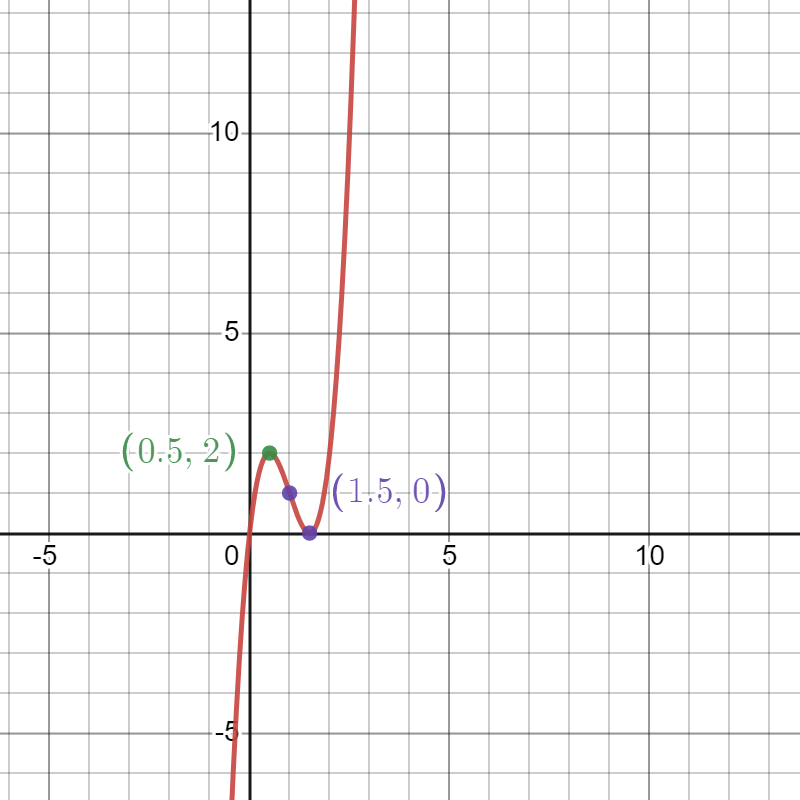
\includegraphics[scale=0.3]{graph_a.png}
    \caption{Graph of V(x) with $a = 3$}
    \label{fig:my_label}
\end{figure}

Here we see that the maximum for $a = 3$ is $x = \frac{1}{2}$ with $V(1/2) = 2$.
\subsection*{Part f}
To find the inflection points of $V(x)$ we compute the following,

\begin{equation*}
   V''(x) = -8(a-3x) = 0
\end{equation*}
we get $x = \frac{a}{3}$ is the inflection point of $V(x)$. Then for $a = 3$, $x = 1$ is the inflection point with $V(x) = 1$

\section*{Question \#2}

\subsection*{Part a}

\begin{figure}[H]
    \centering
    \begin{tikzpicture}
    \draw (0,0) -- node[below, pos=.5]{$a$}(4,0) -- node[right, pos=.5]{$b$}(4,2) -- (0,2) -- (0,0) ;

    \draw (0,0) -- node[below, pos=.5]{$x$}(0.5,0) -- node[right, pos=.5]{$x$}(0.5,0.5) -- (0,0.5) -- (0,0) ;

    \draw (0,1.5) -- (0.5,1.5) -- (0.5,2) -- (0,2) -- (0,1.5) ;

     \draw (3.5,1.5) -- (4,1.5) -- (4,2) -- (3.5,2) -- (3.5,1.5) ;

      \draw (3.5,0) -- (4,0) -- (4,0.5) -- (3.5,0.5) -- (3.5,0) ;
    
    \end{tikzpicture}

    
    \caption{$a \times b$ Square Paper}
    \label{fig:paper}
\end{figure}

\begin{figure}[H]
    \centering
    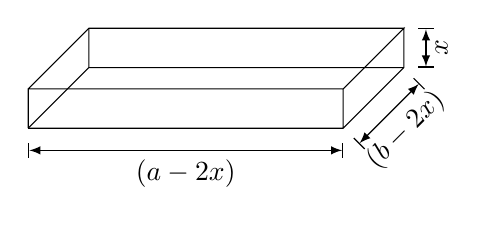
\begin{tikzpicture}[>=latex,scale=2]
    \pgfmathsetmacro{\x}{2}
    \pgfmathsetmacro{\y}{1}
    \pgfmathsetmacro{\z}{0.25}
    \path (0,0,\y) coordinate (A) (\x,0,\y) coordinate (B) (\x,0,0) coordinate (C) (0,0,0)
    coordinate (D) (0,\z,\y) coordinate (E) (\x,\z,\y) coordinate (F) (\x,\z,0) coordinate (G)
    (0,\z,0) coordinate (H);
    \draw (A)--(B)--(C)--(G)--(F)--(B) (A)--(E)--(F)--(G)--(H)--(E);
    \draw (A)--(D)--(C) (D)--(H);
    
    \draw[thin,|<->|] ($(A)+(0,-4pt)$) -- node[below]{$(a-2 x)$}($(B)+(0,-4pt)$);
    \draw[thin,|<->|] ($(B)+(-45:4pt)$) -- node[below,sloped]{$(b-2x)$}($(C)+(-45:4pt)$);
    \draw[thin,|<->|] ($(C)+(4pt,0)$) -- node[below,sloped]{$x$}($(G)+(4pt,0)$);
    
    \end{tikzpicture}
    \caption{Open-Top Box}
    \label{fig:OTB2}
\end{figure}

\subsection*{Part b}
Here we can express the volume of \textbf{Figure \ref{fig:OTB2}} as,

\begin{equation*}
    V(x) = x(a-2x)(b-2x)
\end{equation*}

\subsection*{Part c}

To find the maximum volume of \textbf{Figure \ref{fig:OTB2}} we first compute,

\begin{align*}
    V'(x) &= ab - 4ax-4bx + 12x^2 \\ &= 12x^2 -4x(a+b) + ab = 0
\end{align*}

and by the \textit{quadratic formula}, we get

\begin{align*}
    x_1 &= \frac{1}{6}\left(\sqrt{a^2 - ab + b^2} + a + b\right) \\
    x_2 &= \frac{1}{6}\left(-\sqrt{a^2 - ab + b^2} + a + b\right)
\end{align*}

Next we will find $V''(x)$ by,
\begin{equation*}
    V''(x) = -4(a+b-6x)
\end{equation*}

and plug-in the above roots,

\begin{align*}
    V''(x_1) &= 4 \sqrt{a^2 - ab + b^2}\\
    V''(x_2) &= -4 \sqrt{a^2 - ab + b^2}
\end{align*}

Thus since $V''(x_2) < 0$ we see that at $x_2 = \frac{1}{6}\left(-\sqrt{a^2 - ab + b^2} + a + b\right)$ that $V(x)$ achieves a maximum.

\subsection*{Part d}
\begin{figure}[H]
    \centering
    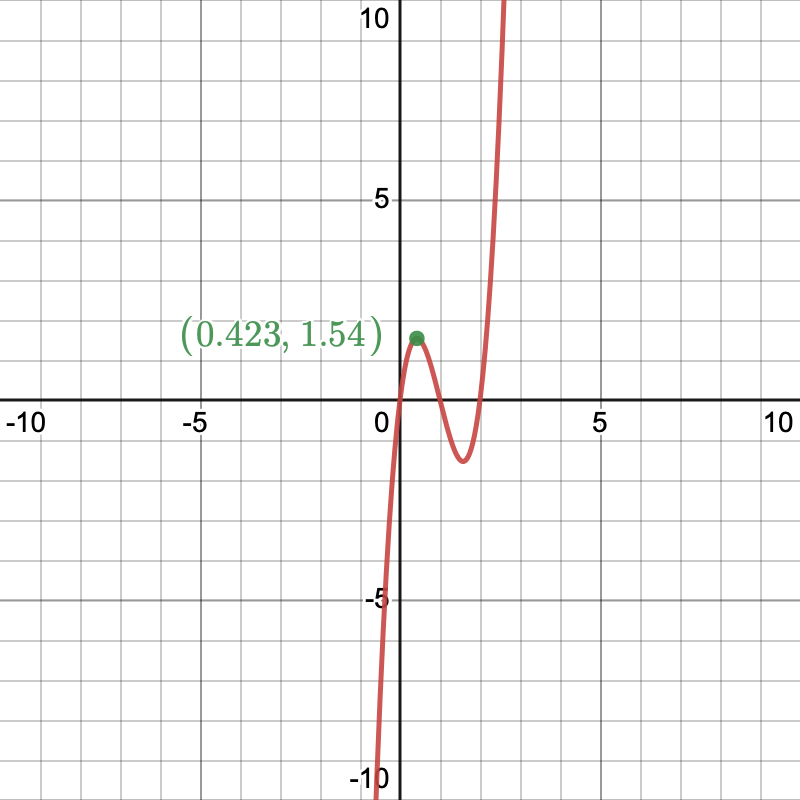
\includegraphics[scale=0.3]{graph_b.png}
    \caption{$V(x)$ with $a = 4$ and $b = 2$}
    \label{fig:my_label}
\end{figure}

\section*{Question \#3}

\subsection*{Part a}
Here from the example in $2D$ we will let $a = 8$in and $b = 6$in for our paper.

\subsection*{Part b}
Here we see that the maximum volume is found as,

\begin{equation*}
    V\left(\frac{1}{6}(14-2\sqrt{13})\text{in}\right) = \frac{8}{27}(35 + 13\sqrt{13})\text{in}^3 \approx 24.258\text{in}^3
\end{equation*}

\subsection*{Part c}
Below is a physical box with $x = \frac{1}{6}(14-2\sqrt{13})\text{in}$
\begin{figure}[H]
    \centering
    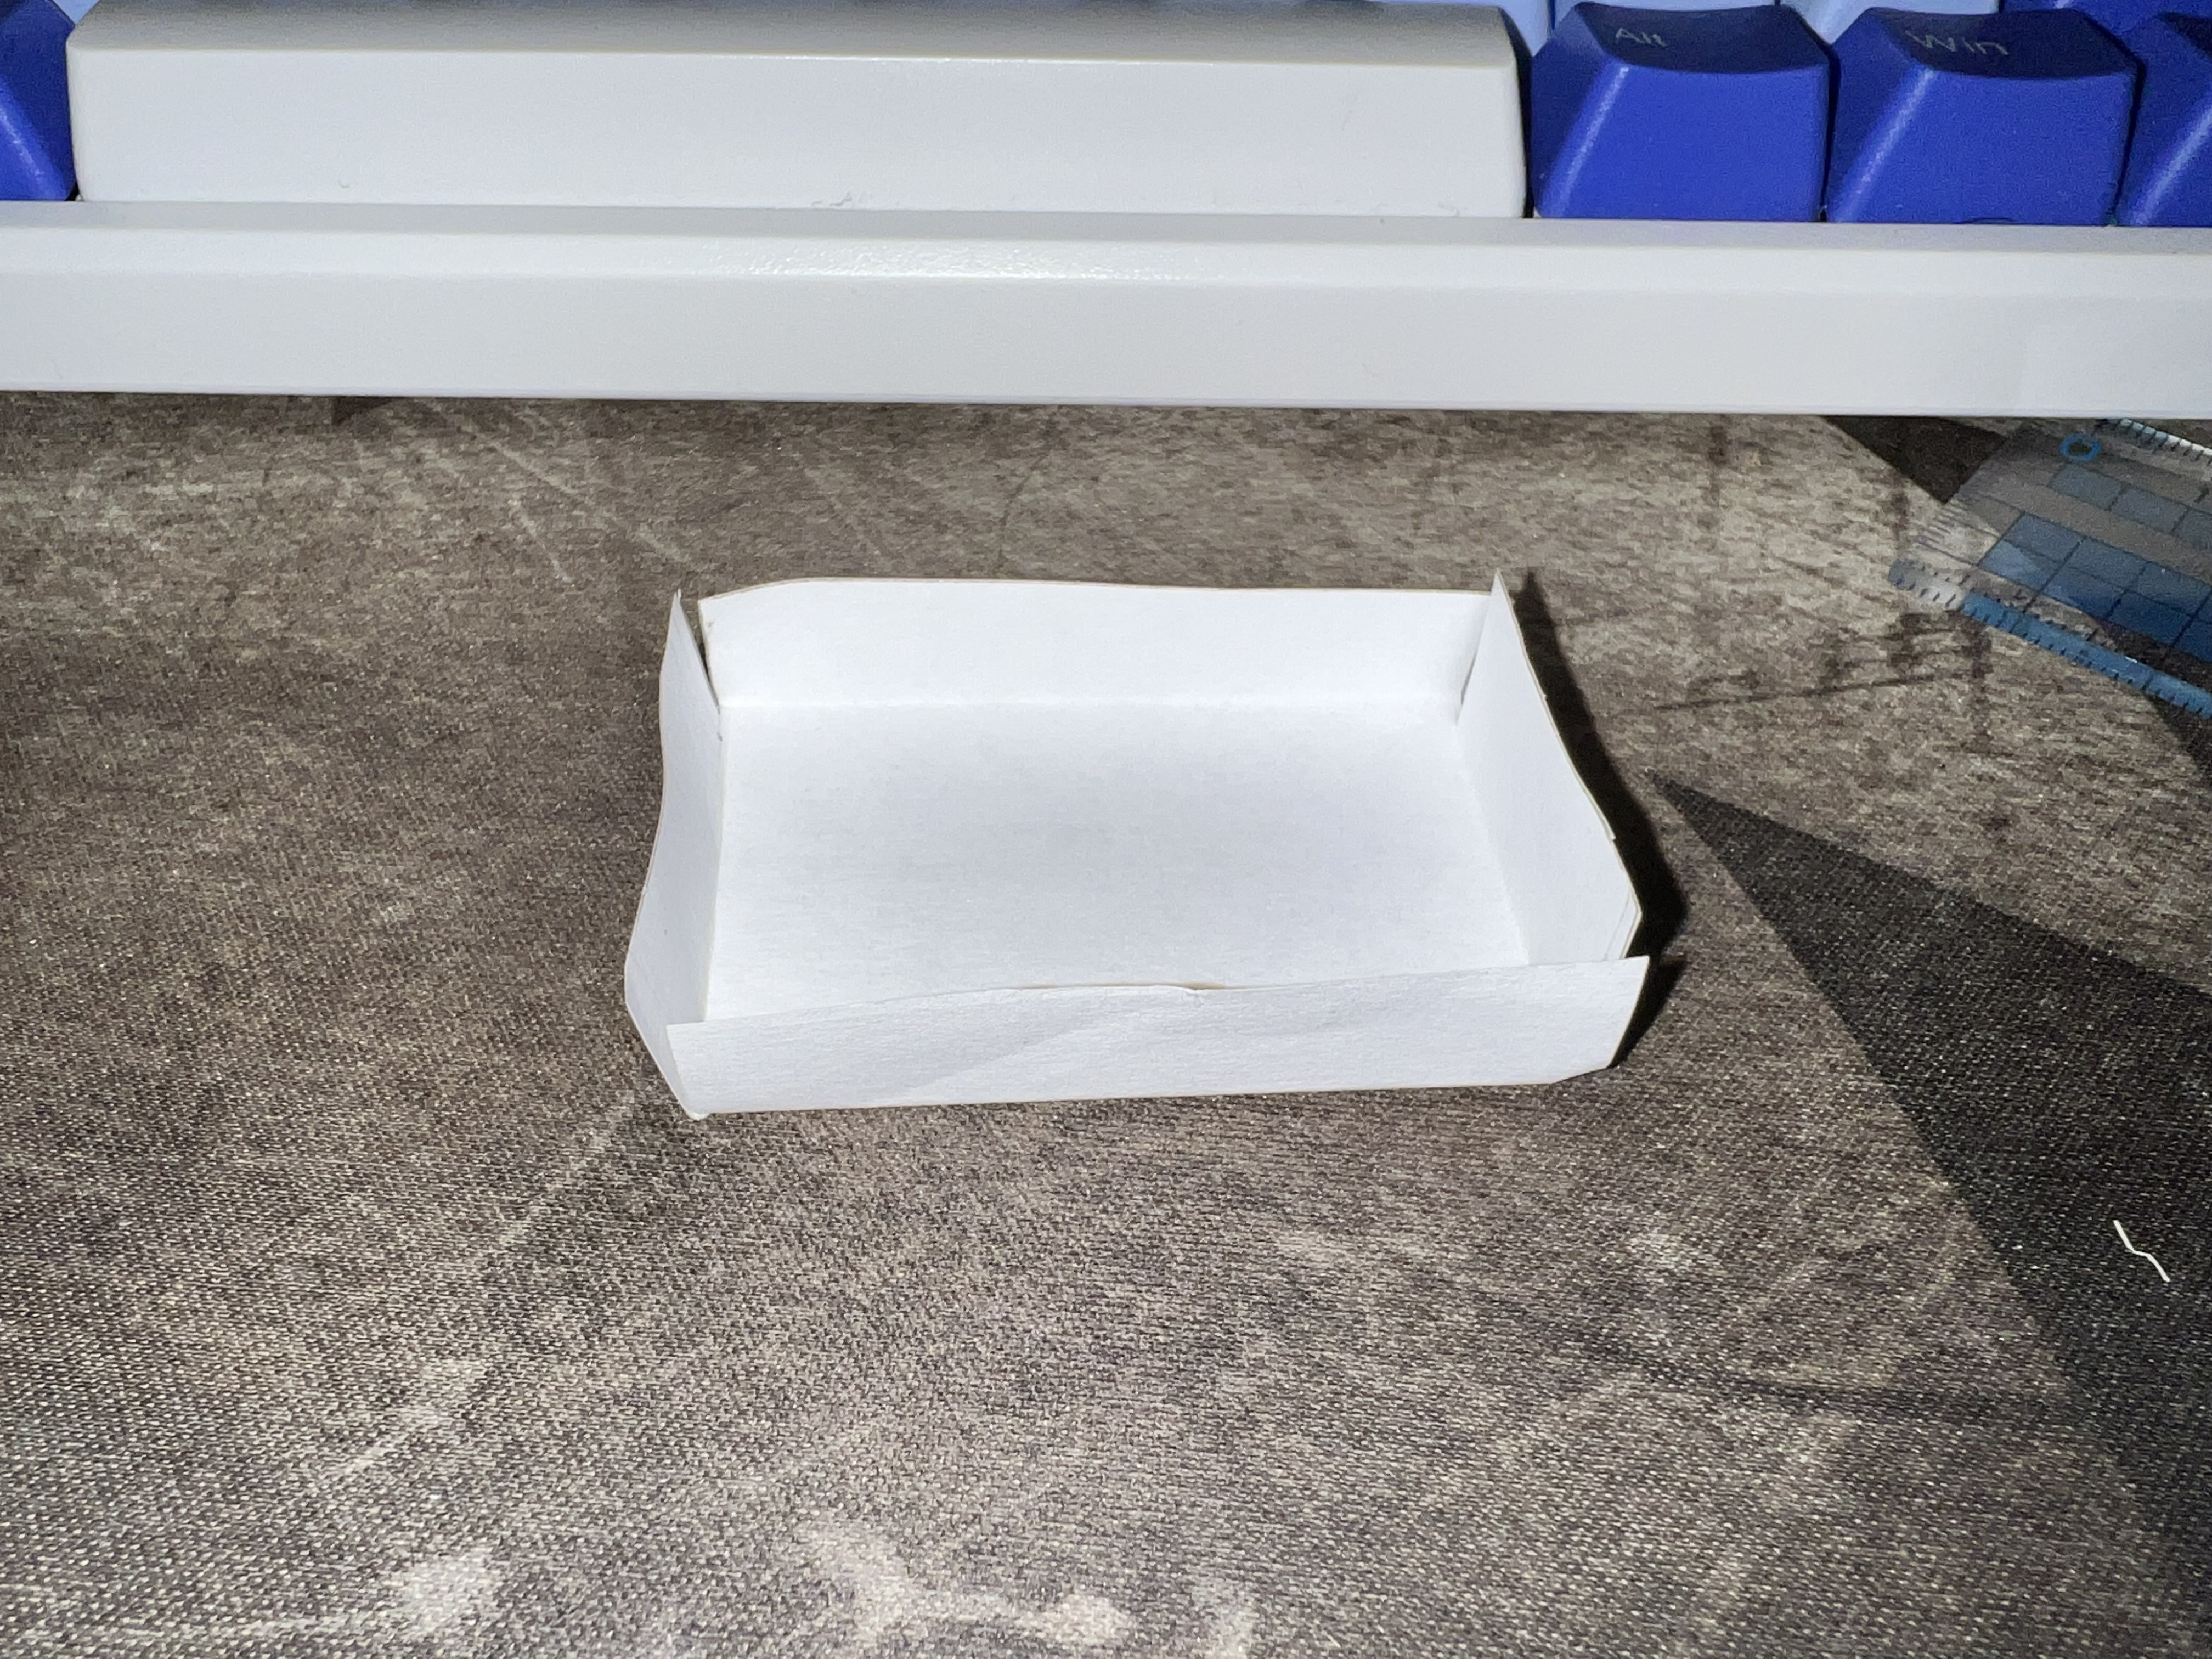
\includegraphics[scale=0.1]{IMG_2255.jpg}
    \caption{$8$in $\times 6$in Open-Top Box (best attempt)}
    \label{fig:my_label}
\end{figure}


\end{document} 